% !TEX root = ../VPJ.tex

\chapter{Schnittstellen}
\label{sec:Schnittstellen}

\inlinetodo{Schnittstellen}

\section{Kommunikation zu Robotinos}
\label{sec:Gewerk2Protokoll}

Die Robotinos werden von Gewerk 2 verwaltet und programmiert. Um eine erfolgreiche Kommunikation zwischen Fertigungsplanungsrechner und Robotino zu gewährleisten existieren folgende Vereinbarungen mit Gewerk 2.

\subsection{Sequenzdiagramm}
\label{sec:sequenzdiagram}

Zunächst wurde eine Struktur entwickelt, in der beschrieben wird, wie die Daten zwischen Robotino und Fertigungsplanungsrechner ausgetauscht werden sollen. Dies wurde anschließend in einem Sequenzdiagramm, Abbildung \ref{fig:Sequenzdiagramm}, dargestellt. 

\begin{figure}[htb]
    \centering
    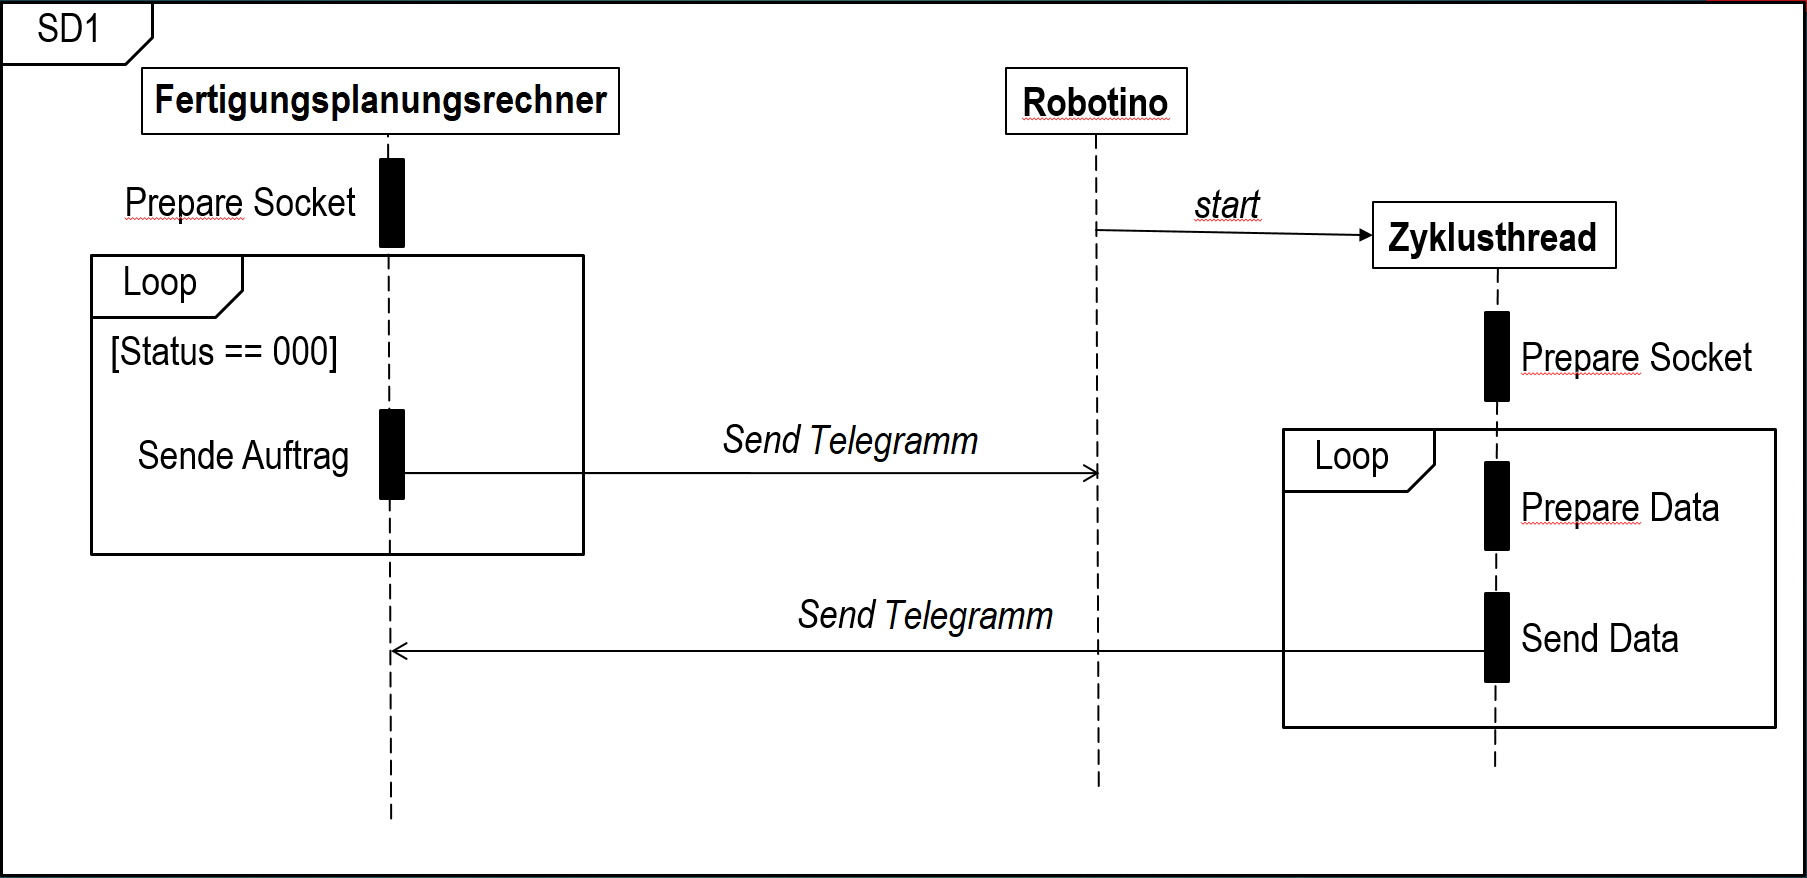
\includegraphics[width=0.9\textwidth]{Abbildungen/Sequenzdiagramm.PNG}
    \caption{Sequenzdiagramm}		
    \label{fig:Sequenzdiagramm}
\end{figure}

Dem Sequenzdiagramm ist zu entnehmen, dass der Robotino nach Programmstart zyklisch Daten sendet. Die Zykluszeit beträgt 100 ms. Da die Daten über UDP an einen spezifizierten Port versendet werden ist ein Empfänger nicht zwangsweise erforderlich und die Programme können unabhängig voneinander laufen. Der Inhalt der Daten ist in Abschnitt \ref{sec:Telegramme} beschrieben. Solange der Robotino läuft werden die Daten gesendet. Dadurch kann auch ein Ausfall der Kommunikation festgestellt werden. 

Auf Seiten des Fertigungsplanungsrechners wird nur bei Bedarf ein Sendevorgang eingeleitet. Erst wenn ein Auftrag an den Robotino gesendet werden soll wird eine Schleife ausgeführt. In der Schleife wird der Auftrag zyklisch an den Robotino gesendet. Die Zykluszeit beträgt hierbei 700 ms. In Kapitel \ref{sec:StateMachineImplementierung} ist die in einer State-Machine implementierte Schleife beschrieben. Die Schleife kann durch Empfangen einer Statusänderung des Robotinos verlassen werden. Dadurch wird eine erfolgreiche Übertragung des Auftrags sichergestellt werden. Die im Auftrag befindlichen Daten sind in Abschnitt \ref{sec:Telegramme} näher erläutert.

\subsection{Telegramme}
\label{sec:Telegramme}

Die Telegramme zwischen Robotino und Fertigungsplanungsrechner bestehen aus einer festgelegten Struktur. Dabei ist sowohl die Länge der Telegramme als auch der Inhalt festgeschrieben. In beiden Telegrammen werden Double-Werte in einem Byte versendet. Jedes Byte muss daher kodiert und dekodiert werden. 

\subsubsection{Telegramm vom Fertigungsplanungsrechner zu Gewerk 2}

Der Auftrag, der an den Robotino gesendet wird, enthält 5 Bytes. Eine Aufschlüsselung ist in Tabelle \ref{tab:TelegrammZuG2} dargestellt. 

\begin{table}[!ht]
	\centering
	\begin{tabular}{|r|c|l|}
		\hline
		Byte & Inhalt	&	Beschreibung \\
		\hline
			1  & Auftragsart & 1: Transport; 2: Parken; 3: Laden  \\
			2  & Position 1  & z.B. 11 \\
			3  & Position 2  & z.B. 32 \\
		  4  & AliveStatus & 1 senden nach Alive Anfrage \\
		  5  & *Reserved   &  \\
		\hline
	\end{tabular}
	\caption{Telegramm zu Gewerk 2}
	\label{tab:TelegrammZuG2}
\end{table}

Das erste Byte klassifiziert die Auftragsart. Diese beschreibt, welche Tätigkeit der Robotino als nächstes tun soll. Auftragsart eins bedeutet, dass der Robotino einen Transportauftrag erhalten hat, also ein Werkstück von einer Position zu einer anderen Position fahren soll. Die Auftragsart 2 zeigt an, dass der Robotino auf einen Parkplatz geschickt wird. Eine Ladefahrt wird mit Auftragsart 3 gekennzeichnet. 

Im zweiten und dritten Byte sind die Positionen angegeben, an welche sich der Robotino bewegen soll. Dabei wird Position 2 nur bei Auftragsart 1 befüllt bzw. ausgewertet, da ein Parken und Laden nur eine Zielposition benötigt. Bei Auftragsart 1 jedoch zeigt Position 1 den Arbeitsplatz an, wo das Werkstück abgeholt werden soll und Position 2 den Ablageort des Werkstücks. 

Über das vierte Byte kann dem Robotino ein Status-Flag gesendet werden. Sobald der Robotino eine Anfrage zu dem Flag sendet wird eine 1 zurückgesendet. Ansonsten ist der Wert 0. Damit kann der Robotino die Funktionalität der Kommunikation validieren.

Mit dem fünften Byte wird eine einfache Erweiterung des Telegramms ermöglicht, sofern mehr Daten übertragen werden sollen. Am Anfang der Ausarbeitung des Projektes war das vierte Byte ebenfalls ein reserviertes Byte. 

\subsubsection{Telegramm von Gewerk 2 zum Fertigungsplanungsrechner}

%00: nichts; 01: unbekanntes Hindernis; 
%02: anderer Roboter; 03: direkt was gesehen?!? (flackert evtl)
%*1   X1: 1: Auf dem Weg; 2: Bin bei…; 
%X2 + X3 : Position 
%1: lebe ich noch? (Antwort senden) 0: ignorieren

\begin{table}[!ht]
	\centering
	\begin{tabular}{|r|c|l|}
		\hline
		Byte & Inhalt	&	Beschreibung \\
		\hline
			1  & Error &  Errortyp  \\
			2  & Akku  & Prozentwert als Integer \\
			3  & Hindernis & Hindernistyp \\
		  4  & *Reserved &  interner Roboterstatus \\
		  5  & AliveAbfrage  & 1: Roboterabfrage erfordert Antwort; 0: egal \\
		  6  & Status & $X_1X_2X_3$; 000: nichts zu tun \\
		  7  & Greifer   & 0:leer; 1:voll \\
		  8  & *Reserved &  \\
		  9  & *Reserved   &  \\
		\hline
	\end{tabular}
	\caption{Telegramm von Gewerk 2}
	\label{tab:TelegrammVonG2}
\end{table}

Robotererrortypen beschreiben

\begin{figure}[htb]
    \centering
    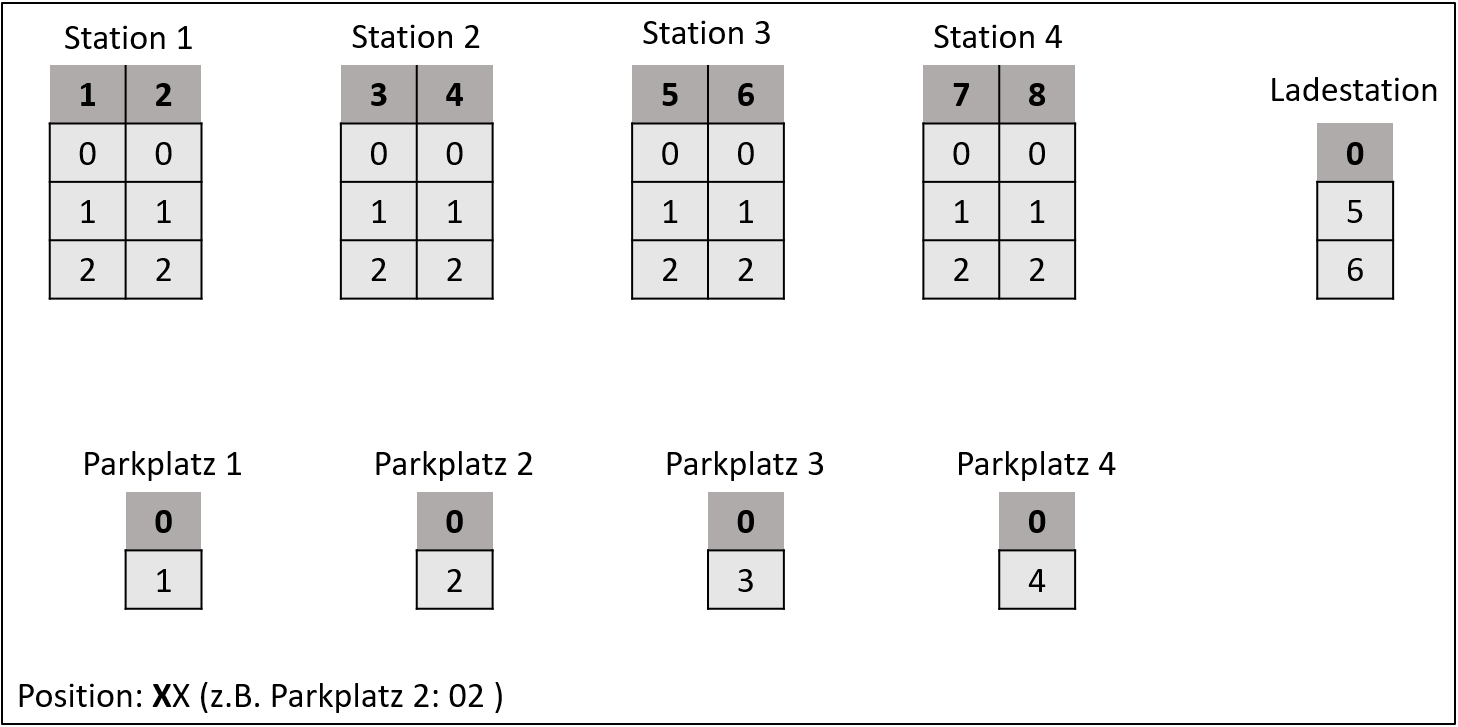
\includegraphics[width=0.9\textwidth]{Abbildungen/Positionskodierung.PNG}
    \caption{Positionskodierung}		
    \label{fig:Positionskodierung}
\end{figure}

Positionskodierung

\inlinetodo{Telegram Gewerk 2}

\inlinetodo{Port vereinbarung}

\subsection{Fehlertypen und Behebung}
\label{sec:Error}

\subsubsection{Fehlertyp 1}
\subsubsection{Fehlertyp 2}
\subsubsection{Fehlertyp 3}
